% !TeX program = lualatex
\documentclass[tikz,border=2pt]{standalone}

\usepackage{pgfplots}
\pgfplotsset{compat=1.18}
\usetikzlibrary{shapes.geometric}
\usepgfplotslibrary{fillbetween}
\usepackage[colorlinks=true,linkcolor=blue,urlcolor=blue]{hyperref}

\pgfdeclareplotmark{mystar}{
  \node[star,star point ratio=2.25,minimum size=10pt,
        inner sep=0pt,draw=black,solid,fill=green] {};
}

\begin{document}

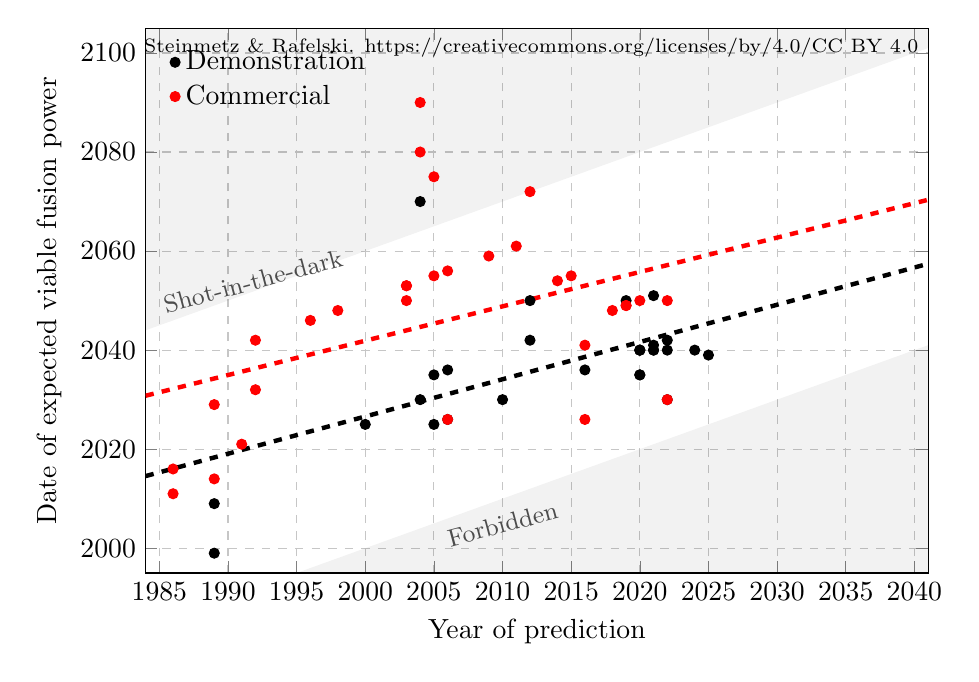
\begin{tikzpicture}
\begin{axis}[
  width=0.95\linewidth,
  height=8.5cm,
  xlabel={Year of prediction},
  ylabel={Date of expected viable fusion power},
  xmin=1984, xmax=2041,
  ymin=1995, ymax=2105,
  major grid style={dashed, gray!45},
  minor grid style={dashed, gray!25},
  xtick={1985,1990,1995,2000,2005,2010,2015,2020,2025,2030,2035,2040},
  xticklabels={1985,1990,1995,2000,2005,2010,2015,2020,2025,2030,2035,2040},
  ytick={2000,2020,2040,2060,2080,2100},
  yticklabels={2000,2020,2040,2060,2080,2100},
  grid=both,
  legend style={at={(0.02,0.98)},anchor=north west,draw=none,fill=none},
  legend cell align=left
]

% Demonstration (black)
\addplot[only marks,mark=*,mark size=1.8pt,black] coordinates {
  (1989,1999) (1989,2009) (2000,2025) (2004,2030) (2004,2070)
  (2005,2025) (2005,2035) (2006,2036) (2006,2026) (2010,2030)
  (2012,2042) (2012,2050) (2016,2036) (2019,2050) (2020,2040)
  (2020,2035) (2020,2040) (2020,2035) (2020,2040) (2021,2040)
  (2021,2040) (2021,2041) (2021,2051) (2022,2030) (2022,2042)
  (2022,2040) (2024,2040) (2025,2039)
};

% Commercial (red)
\addplot[only marks,mark=*,mark size=1.8pt,red] coordinates {
  (1986,2011) (1986,2016) (1989,2014) (1989,2029) (1991,2021)
  (1992,2032) (1992,2042) (1996,2046) (1998,2048) (2003,2050)
  (2003,2053) (2003,2053) (2004,2080) (2004,2090) (2005,2075)
  (2005,2055) (2006,2056) (2006,2026) (2009,2059) (2011,2061)
  (2012,2072) (2014,2054) (2015,2055) (2016,2041) (2016,2026)
  (2018,2048) (2019,2049) (2019,2049) (2020,2050) (2022,2050)
  (2022,2030)
};

% Linear fits
\addplot[black,dashed,line width=1.6pt,domain=1984:2041,samples=2] {0.752*x + 522.6};
\addplot[red,  dashed,line width=1.6pt,domain=1984:2041,samples=2] {0.694*x + 653.9};

% Forbidden: y < x
\addplot[domain=1984:2041,samples=2,draw=none,fill=black,fill opacity=0.05] {x} \closedcycle;

% Shot-in-the-dark: y > x + 60
\addplot[draw=none,fill=black,fill opacity=0.05] coordinates {
  (1984,2105) (2041,2105) (2041,{2041+60}) (1984,{1984+60})
};

\node[font=\small,rotate=15,anchor=north west,text=black!70] at (axis cs:2005,2005) {Forbidden};
\node[font=\small,rotate=15,anchor=south west,text=black!70] at (axis cs:1985,{1985+60}) {Shot-in-the-dark};

\legend{Demonstration,Commercial}

\node[font=\scriptsize, anchor=north east]
at (axis description cs:1.0,1.0)
{\textcopyright\ 2025 Steinmetz \& Rafelski. \href{https://creativecommons.org/licenses/by/4.0/}{CC~BY~4.0}};

\end{axis}
\end{tikzpicture}

\end{document}